\documentclass[10pt, oneside]{article} 
\usepackage{amsmath, amsthm, amssymb, calrsfs, wasysym, verbatim, bbm, color, graphics, graphicx, geometry}
\usepackage[most]{tcolorbox}
\usepackage{xcolor}
\usepackage{framed}
\colorlet{shadecolor}{blue!15}
\graphicspath{ {./} }

\geometry{tmargin=.75in, bmargin=.75in, lmargin=.75in, rmargin = .75in}  

\newcommand{\R}{\mathbb{R}}
\newcommand{\C}{\mathbb{C}}
\newcommand{\Z}{\mathbb{Z}}
\newcommand{\N}{\mathbb{N}}
\newcommand{\Q}{\mathbb{Q}}
\newcommand{\Cdot}{\boldsymbol{\cdot}}

\newtheorem{thm}{Theorem}
\newtheorem{defn}{Definition}
\newtheorem{conv}{Convention}
\newtheorem{rem}{Remark}
\newtheorem{lem}{Lemma}
\newtheorem{cor}{Corollary}
\newtheorem{exa}{Example}

\usepackage{tikz}
\usetikzlibrary{shapes.geometric, arrows}

\tikzstyle{startstop} = [rectangle, rounded corners, 
minimum width=3cm, 
minimum height=1cm,
text centered, 
draw=black, 
fill=red!30]

\tikzstyle{io} = [trapezium, 
trapezium stretches=true, % A later addition
trapezium left angle=70, 
trapezium right angle=110, 
minimum width=3cm, 
minimum height=1cm, text centered, 
draw=black, fill=blue!30]

\tikzstyle{process} = [rectangle, 
minimum width=3cm, 
minimum height=1cm, 
text centered, 
text width=3cm, 
draw=black, 
fill=orange!30]

\tikzstyle{decision} = [diamond, 
minimum width=3cm, 
minimum height=1cm, 
text centered, 
draw=black, 
fill=green!30]
\tikzstyle{arrow} = [thick,->,>=stealth]


\title{Hidr\'aulica B\'asica [2015961] \\ \textbf{Tema \# 2: An\'alisis de sistemas de tuber\'ias}}
\author{\textbf{Luis Alejandro Morales (Ph.D)}\\ \vspace{0.4cm} Profesor Asistente \\ Universidad Nacional de Colombia-Bogot\'a\\Facultad de Ingenier\'ia \\ Departamento de Ingenieria Civil y Agr\'icola}
%\date{Periodo 2023-II}
\date{}

\begin{document}

\maketitle
\tableofcontents

%\vspace{.25in}

%%%%%%%%
\section{Sistemas de tuber\'ias simples} 
Una tuber\'ia simple es aquella que tiene un di\'ametro y esta hecha de un solo material a lo largo de su longitud. La energ\'ia que mueve el flujo dentro de la tuber\'ia es gracias a la acci\'on de la gravedad (tanque a la entrada) o a un m\'aquina (sistema de bombeo a la entrada). Dichas tuber\'ias pueden tener cualquier tipo de accesorio a lo largo de su longitud lo que implica unas p\'erdidas menores. Las ecuaciones de Prandl, Von-Karman y Darcy-Weisbach vistas en la Unidad 1, son utilizadas para el dise\~no de tuber\'ias simples. Note que existe cierta dificultad para el disen\~no teniendo en cuenta que la ecuaci\'on de Colebrook-White para calcular el coeficiente de rugosidad $f$ es implicita y requiere un proceso iterativo para su soluci\'on. Los algoritmos que aqu\'i se discutir\'an, constituyen las bases para el an\'alisis y dise\~no de tuber\'ias m\'as complejos. 

\subsection{Tipos de problema en sistemas de tuber\'ias}
Los problemas en sistemas de tuber\'ias se clasifican de acuerdo con las variables desconocidas. Las variables involucradas en estos problemas se pueden clasificar como:
\begin{itemize}
\item \emph{Caracter\'isticas la tuber\'ia}: Di\'ametro ($D$), longitud ($L$), rugosidad absoluta ($\varepsilon$).
\item \emph{Propiedades del fluido}: Densidad ($\rho$) y viscosidad din\'amica ($\mu$). 
\item \emph{Variables relacionadas con el esquema del sistema}: Coeficientes de p\'erdidas menores ($K$) de todos los accesorios en el sistema. 
\item \emph{Variables relacionas con la energ\'ia impulsora del sistema}: Cabeza de energ\'ia ($H$) entre el embalse de entrada y la salida del sistema, o potencia de la bomba ($P$). 
\item \emph{Propiedades del flujo}: Caudal ($Q$) y velocidad ($V$) del flujo.
\item \emph{Otras variables}: Aceleraci\'on de la gravedad ($g$).
\end{itemize}
 
De acuerdo con las variables involucradas en sistemas de tuber\'ias, existen tres tipos de problemas:
\begin{enumerate}
\item \textbf{Comprobaci\'on de dise\~no}: En este tipo de problemas la tuber\'ia existe y se conoce su longitud, su di\'ametro, su rugosidad absoluta (material), al igual que todos los accesorios y sus coeficiente de p\'erdidas menores. Tambi\'en se conoce la energ\'ia impulsora, ya sea una cabeza de energ\'ia (gravitacional por diferencia de niveles) o una energ\'ia mec\'anica (suministrada por una bomba). Las propiedades del fluido como la densidad y la viscosidad absoluta son tambi\'en conocidas. La incognita es entonce el caudal o la velocidad del flujo en el sistema.
\begin{table}[h!]
\centering
\begin{tabular}{c c}
 \hline
 Variables conocidas & Inc\'ognita \\ [0.5ex]
% \hline\hline
D, $\varepsilon$, H (o P), $\sum K$, $\rho$, $\mu$, g, L & Q (o V) \\
\hline
\end{tabular}
%\caption{Coeficientes de rugosidad de Hazen-Williams, $C_H$ (tomado de \cite{agudelo2011mecanica}).}
%\label{hwi}
\end{table}
 
\item \textbf{C\'alculo de la potencia requerida}: En este tipo de problemas, el sistema existe por lo que se conocen su longitud, su di\'ametro, su rugosidad absoluta (material), al igual que todos los accesorios y sus coeficiente de p\'erdidas menores. Las propiedades del fluido como la densidad y la viscosidad din\'amica as\'i como el caudal (o velocidad) que fluye por el sistema son tambi\'en conocidas. La finalidad es determinar la potencia, ya sea mec\'anica o gravitacional, requerida para mover cierto caudal a trav\'es de la tuber\'ia dada. 

\begin{table}[h!]
\centering
\begin{tabular}{c c}
 \hline
 Variables conocidas & Inc\'ognita \\ [0.5ex]
% \hline\hline
D, $\varepsilon$, Q (o V), $\sum K$, $\rho$, $\mu$, g, L & P (o H) \\
\hline
\end{tabular}
%\caption{Coeficientes de rugosidad de Hazen-Williams, $C_H$ (tomado de \cite{agudelo2011mecanica}).}
%\label{hwi}
\end{table}
 
\item \textbf{Dise\~no de la tuber\'ia}: En este tipo de problemas se conoce el caudal o la velocidad de flujo y la potencia disponible (mec\'anica o gravitacional), algunas caracter\'isticas de la tuber\'ia como la longitud, los accesorios y sus coeficientes de p\'erdida y las propiedades del fluido como la densidad y la viscosidad din\'amica. Se desconoce el di\'ametro necesario para permitir el paso de el caudal demandado. En cuanto a la rugosidad absoluta, se debe cambiar el tipo de tuber\'ia (rugosidad absoluta) con el fin de obtener la mejor opci\'on. 

\begin{table}[h!]
\centering
\begin{tabular}{c c}
 \hline
 Variables conocidas & Inc\'ognita \\ [0.5ex]
% \hline\hline
$\varepsilon$, Q (o V), P (o H), $\sum K$, $\rho$, $\mu$, g, L &  D \\
\hline
\end{tabular}
%\caption{Coeficientes de rugosidad de Hazen-Williams, $C_H$ (tomado de \cite{agudelo2011mecanica}).}
%\label{hwi}
\end{table}
 \end{enumerate}

\subsection*{Ecuaciones para la soluci\'on de problemas}
%Si se tiene el sistema de la figura~\ref{comp1}, la ecuaci\'on de Bernoulli entre los puntos 1(entrada) y 2(salida) es:
A continuacion se presentan las ecuaciones necesarias para resolver los tres problemas ya mencionadas. Estas ecuaciones fueron discutidas en el capitulo anterio. 

Si se tiene una tuber\'ia simpre cuya entrada es en la secci\'on 1 y cuya salida es en la secci\'on, aplicando la ecuacion de Bernoulli entre 1 y 2, de manera general,  se tiene:

% Fig 2.4 from Salda 
%\begin{figure}[h]
%\centering
%\includegraphics[width=8cm]{comp1.jpeg}
%\caption{Tuber\'ia simple alimentada por un tanque de nivel constante y con descarga a la atmosfera (tomado de \cite{saldarriaga}).} 
%\label{ttub}
%\end{figure}

\begin{equation}
\frac{{V_1}^2}{2g}+ z_1 + \frac{p_1}{\gamma} =  \frac{{V_2}^2}{2g}+ z_2 + \frac{p_2}{\gamma} + h_f + \sum h_e - h_b + h_t
\label{com1}
\end{equation}

donde $h_b$ es la cabeza de energ\'ia suministrada por la bomba y $h_t$ es la cabeza de energ\'ia sustraida por la turbina. La energia total en una seccion (e.g. 1 o 2) de flujo se puede expresar como $E = \frac{{V}^2}{2g}+ z + \frac{p}{\gamma}$, por lo tanto la ecuaci\'on~\ref{com1} se puede expresar como:

\begin{equation}
E_1 - E_2 = h_f + h_e - h_b + h_t
\label{com1a}
\end{equation}

en donde $h_f$ son las p\'erdidas por fricci\'on   estimadas con la ecuaci\'on de Darcy-Weisbach como:

\begin{equation}
\color{red}\boxed{\color{black} h_f = f \frac{L}{D}\frac{V^2}{2g} }
\label{com2}
\end{equation}

y $h_e$ son las perdidas por accesorios, las cuales se pueden calcular como:

\begin{equation}
\color{red}\boxed{\color{black} h_e = \sum K \frac{V^2}{2g} }
\label{com3}
\end{equation}

El factor de fricci\'on $f$ en la ecuacio\'on~\ref{com2}, se calcula usando el diagrama de Moody o numericamente usando la ecuaci\'on Colebrook-White como:
 
\begin{equation}
\color{red}\boxed{\color{black}  \frac{1}{\sqrt{f}}= -2 \log \left( \frac{\varepsilon}{3.7D} + \frac{2.52}{Re \sqrt{f}} \right) }
\label{com4}
\end{equation}

donde el n\'umero de Reynolds ($Re$) se calcula como

\begin{equation}
\color{red}\boxed{\color{black} Re = \frac{VD}{\nu} } 
\label{com5}
\end{equation}

Si se reemplaza las ecuaciones~\ref{com2} y ~\ref{com3} en la ecuaci\'on~\ref{com1a}, se tiene:

\begin{equation}
E_1 - E_2 =  f \frac{L}{D}\frac{V^2}{2g} + \sum K \frac{V^2}{2g} - h_b + h_t
\label{com6}
\end{equation}

despejando $V$ en la ecuaci\'on~\ref{com6}, se tiene:
 
\begin{equation}
\color{red}\boxed{\color{black} V = \sqrt{2g\frac{E_1 - E_2 + h_b - h_t}{f\frac{L}{D} + \sum K } } }
\label{com7}
\end{equation}

En los tres tipos de problemas, el objetivo es usar las ecuaciones~\ref{com2}, ~\ref{com3}, ~\ref{com4}, ~\ref{com5} y ~\ref{com7} para su soluci\'on. Note que la ecuaci\'on~\ref{com4} es una ecuaci\'on implicita que requiere del uso de algun m\'etodo iterativo o numerico para su soluci\'on. Note que la ecuaci\'on~\ref{com7} se usa en particular para la soluci\'on de problemas de \emph{comprobaci\'on de dise\~no} y de \emph{dise\~no de tuber\'ias}.







%donde $H$ es la altura de la superficie de agua del tanque o la energ\'ia total en el punto 1. Teniendo en cuenta que la tuber\'ia del sistema en la figura~\ref{comp1} descarga a la atmosfera, la velocidad as\'i como la presi\'on se vuelven cero ($\frac{{V_2}^2}{2g}= 0$, $\frac{p_2}{\gamma}=0$). Note que la velocidad no necesariamente es cero cuando descarga a la atm\'osfera; se supone entonces que esta \'es cero all\'i.  Como consecuencia de esto, se asume que existen p\'erdidas menores en la salida de la tuber\'ia. La ecuaci\'on~\ref{com1} queda entonces como:
%
%\begin{equation}
%H = z_2 + h_f + \sum h_e 
%\label{com2}
%\end{equation}
%
%Despejando de la ecuaci\'on~\ref{com2}, las p\'erdidas por fricci\'on se pueden calcular como: 
%
%\begin{equation}
%\color{red}\boxed{\color{black} h_f = H - z_2 - \sum K \frac{{V_2}^2}{2g} }
%\label{com3}
%\end{equation}
%
%Mediante la ecuaci\'on de Darcy-Weisbach, despejando el factor de fricci\'on se tiene que:
%
%\begin{equation}
%f = \frac{h_f D 2g}{L V^2}
%\label{com4}
%\end{equation}
%
%Sacando ra\'iz cuadrada e invirtiendo los t\'erminos a ambos lados se tiene:
%
%\begin{equation}
%\frac{1}{\sqrt{f}} = \frac{V\sqrt{L}}{\sqrt{h_f D 2g}}
%\label{com5}
%\end{equation}
%
%Igualando a la ecuaci\'on de Colebrook y  White:
%
%\begin{equation}
% \frac{1}{\sqrt{f}}= -2 \log \left( \frac{\varepsilon}{3.7D} + \frac{2.52}{Re \sqrt{f}} \right) 
%\label{comp6}
%\end{equation}
%
%se tiene:
%
%\begin{equation}
%\frac{V\sqrt{L}}{\sqrt{h_f D 2g}}= -2 \log \left( \frac{\varepsilon}{3.7D} + \frac{2.52}{Re \sqrt{f}} \right) 
%\label{comp7}
%\end{equation}
%
%Reemplazando $Re = \frac{VD}{\nu}$ en la ecuaci\'on~\ref{comp7} y despejando la velocidad, se tiene:
%
%\begin{equation}
%\color{red}\boxed{\color{black} V= \frac{-2\sqrt{2gD h_f}}{\sqrt{L}} \log \left( \frac{\varepsilon}{3.7D} + \frac{2.52 \nu \sqrt{L}}{D \sqrt{2gD h_f}} \right) }
%\label{comp8}
%\end{equation}
%
%La ecuaci\'on~\ref{comp8} es explicita para la velocidad y es utilizado para la soluci\'on de los tres tipos de problemas mencionados hasta el momento. 

\subsection{Solucio\'on de la ecuaci\'on de Colebrook-White}
\subsubsection*{Metodo de punto fijo}
Consiste en el siguiente procedimiento:
\begin{enumerate} 
\item Leer la informacion de entrada: $\varepsilon$, $\rho$, $\mu$ o $\nu$, $V$, $D$ 
\item Asumir un valor inicial de $f_i$ (e.g. $f=0.01$).
\item Usando la siguiente forma de la ecuaci\'on~\ref{com4}, calcular otro valor $f_{i+1}$:

\begin{equation}
\color{red}\boxed{\color{black}  f_{i+1} = \left[-2 \log \left( \frac{\varepsilon}{3.7D} + \frac{2.52}{Re \sqrt{f_i}} \right) \right]^{-2}}
\label{com8}
\end{equation}

\item Si $f_{i}- f_{i+1} \leq \eta$, donde $\eta$ es un error  (e.g. $\eta$ = 1x10$^{-6}$), la iteraci\'on para y va a 6..Si $f_{i}- f_{i+1} \gt \eta$ se calcula un nuevo valor $f_{i+1}$.
\item Imprimir $f$

\end{enumerate} 


\subsection{Comprobaci\'on de dise\~no}
Teniendo en cuenta las ecuaciones de la secci\'on anterion, el procedimiento para determinar el valor de $V$ o $Q$ es:
\begin{enumerate} 
\item Leer la informacion de entrada: $\varepsilon$, $\rho$, $\mu$ o $\nu$, $L$, $D$, $\sum K$, $E1$, $E2$, $h_b$ y $h_t$.
\item Asumir un valor inicial de $f$ (e.g. $f=0.01$).
\item Calcular $V$ usando la ecuaci\'on~\ref{com7}.
\item Calcular $Re$ usando la ecuacion~\ref{com5}.
\item 
\end{enumerate} 

En este tipo de problemas, la supocisi\'on m\'as importante es que $h_f = H$, es decir que la energ\'ia disponible en el sistema se pierde debido a la fricci\'on.
% DF 1 from Salda 
\begin{figure}[h]
\centering
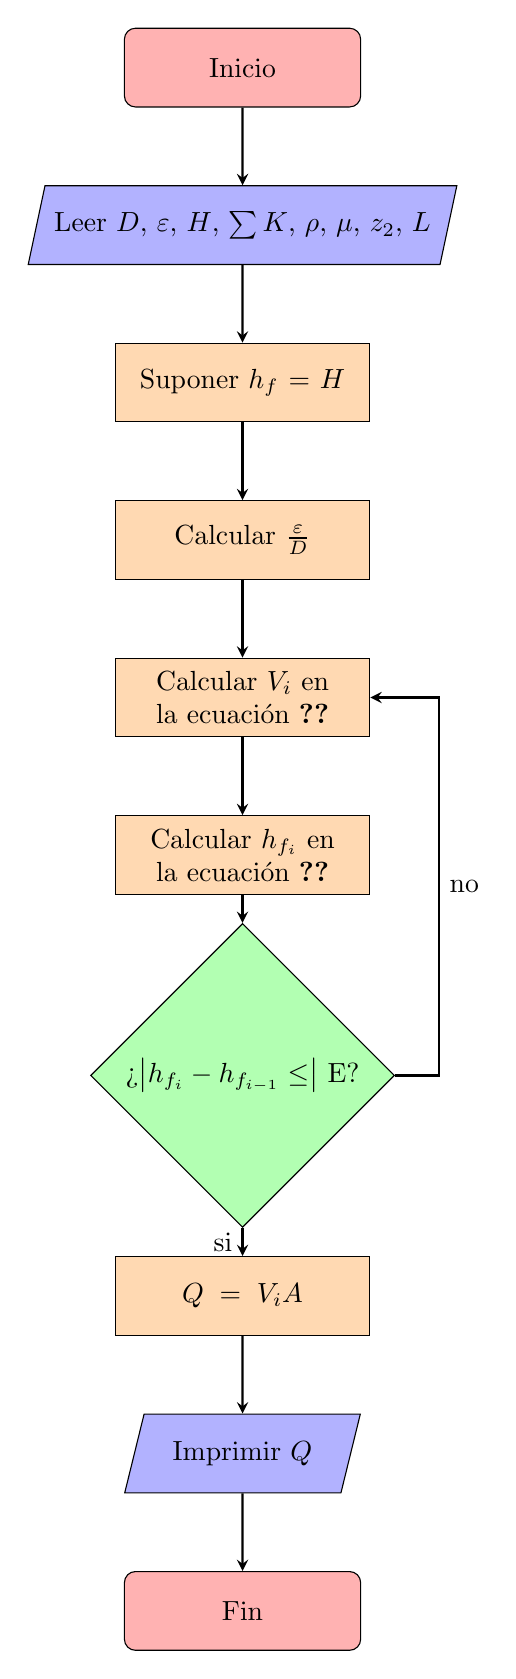
\begin{tikzpicture}[node distance=2cm]

\node (start) [startstop] {Inicio};
\node (in1) [io, below of=start] {Leer $D$, $\varepsilon$, $H$, $\sum K$, $\rho$, $\mu$, $z_2$, $L$};
\node (pro1) [process, below of=in1] {Suponer $h_f = H$};
\node (pro2) [process, below of=pro1] {Calcular $\frac{\varepsilon}{D}$};
\node (pro3) [process, below of=pro2] {Calcular $V_i$ en la ecuaci\'on~\ref{comp8}};
\node (pro4) [process, below of=pro3] {Calcular $h_{f_i}$ en la ecuaci\'on~\ref{com3}};
\node (dec1) [decision, below of=pro4, yshift=-0.8cm] {¿$\left| h_{f_i} - h_{f_{i-1}}\leq \right|$ E?};

%\node (pro2b) [process, right of=dec1, xshift=2cm] {Process 2b};
\node (pro5) [process, below of=dec1, yshift=-0.8cm] {$Q = V_i A$};
\node (out1) [io, below of=pro5] {Imprimir $Q$};
\node (stop) [startstop, below of=out1] {Fin};

\draw [arrow] (start) -- (in1);
\draw [arrow] (in1) -- (pro1);
\draw [arrow] (pro1) -- (pro2);
\draw [arrow] (pro2) -- (pro3);
\draw [arrow] (pro3) -- (pro4);
\draw [arrow] (pro4) -- (dec1);
\draw [arrow] (dec1)   -- ++(2.5,0)  |- (pro3) node[near start, anchor=west] {no};
\draw [arrow] (dec1) -- node[anchor=east] {si} (pro5);
%\draw [arrow] (pro2b) |- (pro1);
\draw [arrow] (pro5) -- (out1);
\draw [arrow] (out1) -- (stop);

\end{tikzpicture}

\caption{Diagrama de flujo para comprobaci\'on de dise\~no (adaptado de \cite{saldarriaga})}
\label{dflow1}
\end{figure}

En la figura~\ref{dflow1} $E$ representa un error que debe ser determinado por el modelador (e.g. 1x10$^{-5}$). Este procedimiento es aplicable a cualquier problema de comprobaci\'on de dise\~no para cualquier sistema de tuber\'ia simple.


\subsubsection*{C\'alculo de la potencia requerida}
\subsubsection*{Disen\~o de la tuber\'ia}
 
%%%%%%%%
\section{Sistemas de tuber\'ias en serie} 

%%%%%%%%
\section{Sistemas de tuber\'ias en paralelo} 

%%%%%%%%
\section{Sistemas de tuber\'ias ramificadas} 

%%%%%%%%
\section{Redes de distribuci\'on: M\'etodo de an\'alisis de Cross}

%%%%%%%%
\section{Redes de distribuci\'on: M\'etodo de an\'alisis lineal}




% REFERENCES
\bibliographystyle{plain} % We choose the "plain" reference style
\bibliography{refs} % Entries are in the refs.bib file



\end{document}
